Receiver Operating Characteristic - Area Under Curvev  is a performance metric for binary classification problems, measuring 
how well a model separates positive and negative classes across all possible probability thresholds
% Suggested packages for the main paper preamble:
% \usepackage{booktabs}
% \usepackage{longtable}
% \usepackage{tabularx}
% \usepackage{tikz}
% \usepackage{pgfplots}
% \pgfplotsset{compat=1.18}
% \usetikzlibrary{arrows.meta,positioning,shapes.geometric}

\section{Abstract}
Logistics routing in small and medium transport operations is still frequently performed using map-based single-trip navigation tools or manual spreadsheet planning. Such approaches are insufficient when shipment decisions must simultaneously consider route time, delay risk, transport cost, and estimated carbon emissions. This work presents an intelligent routing prototype for multi-modal transport systems that combines a FastAPI backend, a React-based control-tower dashboard, PostgreSQL/PostGIS data storage, OSRM-backed road routing, and a machine-learning microservice for delay prediction. The existing system in practice is represented by road-only, single-trip planning with no explicit delay-risk or emissions-aware optimisation. The proposed system extends this by introducing an evaluation framework across road, rail, sea, and air transport strategies, a graph-based multimodal routing prototype, event ingestion for traffic and weather disruption, and a delay-aware decision layer. 

For road segments, shortest-path geometry and travel duration are obtained from OSRM over OpenStreetMap data. For rail, sea, and air, the current prototype uses a graph-search routing layer over a seeded multimodal edge network rather than external operator timetables. Delay modelling is implemented using a Random Forest classifier and Random Forest regressor trained on a 200-row shipment dataset with operational and environmental features. Experimental results show differentiated transport choices under different scenarios: road under short normal trips, rail under congestion and weather conditions, air under peak-hour delay-sensitive conditions, and sea under green-corridor sustainability-weighted conditions. The prototype demonstrates that an emissions-aware and delay-aware multimodal decision-support system can be built as a credible research platform, while also highlighting the gap between a research-grade comparative engine and a fully operational real-world multimodal routing stack.

\section{Introduction}
Modern logistics systems operate in conditions where route planning is no longer a shortest-path problem alone. Transport planners must balance service time, expected disruption, operating cost, and environmental impact while handling shipments across depots, rail yards, ports, airports, and customer delivery points. Prior survey work shows that multimodal transport research has increasingly shifted from single-criterion path finding toward integrated decision models that combine cost, time, network structure, and sustainability concerns \cite{matei2021}. Existing commercial map tools are highly effective for point-to-point road navigation, but they do not natively expose organisation-specific logistics networks, multimodal transfer points, or explicit sustainability trade-offs. As a result, many logistics decisions continue to rely on manual planning or fragmented decision support.

Recent literature confirms that the field is moving in three complementary directions. The first direction focuses on multimodal network design and route selection under multiple objectives, including cost, time, carbon, and risk \cite{ghaderi2015, shang2021, maneengam2023, liwang2023, koohathongsumrit2024}. The second direction focuses on predictive intelligence, especially short-term travel time and disruption-aware route prediction using machine learning \cite{qiu2021, prakash2024}. The third direction extends optimisation to mode-specific domains such as maritime routing, where time, fuel, and emissions are explicitly traded off \cite{zhao2024}. This work addresses that gap by developing a prototype intelligent route optimisation system for multi-modal transport. The prototype is designed as a research platform rather than a production transport management system. Its main objective is to evaluate how transport mode selection changes when travel time, delay risk, cost, and estimated \(\mathrm{CO_2e}\) emissions are jointly considered. The system integrates a backend API, dashboard visualisation, delay prediction service, road routing through OSRM, and a graph-based multimodal routing layer for research scenarios involving rail, sea, and air.

The contribution of this work is threefold. First, it provides an end-to-end software prototype connecting routing, monitoring, event ingestion, and machine-learning-based delay estimation. Second, it introduces an emissions-aware and delay-aware multimodal evaluation workflow that can be executed reproducibly. Third, it provides a controlled set of scenario outcomes that can be used to discuss trade-offs relevant to sustainable development, especially in the context of cleaner freight movement and resilient transport planning. In contrast to optimisation-only studies, the present system also exposes the outputs through a working dashboard; in contrast to purely predictive studies, it carries route and disruption features forward into planning decisions.

\subsection{Existing System}
The existing system, as represented in current industry practice, is dominated by road-only trip planning and static dispatch logic. In many small and medium logistics operations, route choice is produced either manually or with general navigation platforms that optimise one trip at a time. Such tools are useful for driver guidance, but they typically do not integrate shipment priority, estimated disruption, explicit carbon metrics, or alternative transport strategies such as rail, air, or sea. This results in three important limitations: first, decision-making becomes reactive rather than analytical; second, sustainability is rarely quantified in day-to-day routing; and third, multimodal planning remains inaccessible without specialised commercial software.

\subsection{Proposed System}
The proposed system is a multimodal decision-support prototype that extends road navigation with three additional capabilities. The first is \textit{comparative optimisation}, where multiple transport modes are evaluated under the same objective function. The second is \textit{delay-aware planning}, where route and plan decisions can be informed by a machine-learned delay estimate. The third is \textit{operational visibility}, where the selected route, route metrics, recent events, and evaluation indicators are exposed through a dashboard rather than hidden inside a backend service. Although the present prototype does not yet provide timetable-validated real-world rail, sea, or air engine integrations, it does implement these modes as graph-search alternatives over a seeded logistics network, which is sufficient for controlled research comparisons.

\section{Literature Survey}
The verified literature most relevant to this project can be grouped into four themes: multimodal optimisation surveys, multimodal route and hub optimisation, predictive delay and travel-time modelling, and sustainability-oriented routing. These themes map directly to the implemented prototype, which combines a route engine, a comparative optimiser, and a delay prediction service.

Matei et al. surveyed integrative multimodal transport research and showed that the field consistently revolves around the joint treatment of cost, time, and network topology rather than isolated shortest-path planning \cite{matei2021}. That survey is especially relevant to the present project because it highlights the persistent gap between algorithmic models and deployable multimodal software systems. Our prototype explicitly tries to narrow that gap by combining a runnable software stack with a measurable evaluation workflow.

Ghaderi and Pahlavani proposed a multimodal multi-criteria route planning model that combined fuzzy-AHP weighting with simulated annealing \cite{ghaderi2015}. Their case study covered central Tehran and considered five transport modes with fare, time, user discomfort, and path length as criteria. The reported outcome was that the proposed approach achieved high efficiency and speed in identifying acceptable routes. This paper aligns closely with our weighted mode-selection logic because both systems treat route choice as a multi-criteria compromise rather than a single-metric optimum.

Shang et al. studied the bi-objective hierarchical multimodal hub location problem for cargo delivery systems \cite{shang2021}. Using the Turkish network data set, they formulated a mixed-integer model that minimizes both system-wide cost and maximum delivery time, then solved larger instances using variable neighborhood search and an improved NSGA-II. Their results showed that the developed heuristics outperformed a standard NSGA-II on realistic-sized instances. This is directly relevant to our work because it illustrates the kind of stronger hub- and network-level optimiser that would be needed to move our current prototype beyond per-scenario comparative mode selection.

Maneengam addressed a real-world multimodal bulk transportation problem in Thailand using an adaptive \(\varepsilon\)-constraint method to generate Pareto solutions, D-CRITIC to weight the criteria, and modified TOPSIS to rank the alternatives \cite{maneengam2023}. The study simultaneously optimized cost, transport time, and \(\mathrm{CO_2e}\) emissions and reported that the proposed approach produced more Pareto solutions per unit of computational effort than a more conventional \(\varepsilon\)-constraint workflow. This paper is strongly aligned with our current objective formulation because our prototype also compares cost, delay, and emissions together, although with a lighter-weight heuristic implementation.

Li and Wang extended multimodal planning to carbon-aware hub location by formulating a mixed-integer nonlinear model and solving it with an adaptive genetic algorithm \cite{liwang2023}. Their real-world case study around Ningbo Port showed that an additional secondary hub increased cargo flow by 41.46\%, reduced transportation time by 2.2\%, and reduced total cost by 2.35\%. This work is particularly relevant to the SDG framing of our paper because it demonstrates that carbon-aware multimodal decisions can be linked to infrastructure and flow design rather than only to route ranking.

Koohathongsumrit et al. proposed an integrated fuzzy hierarchy risk assessment and multi-criteria decision-making framework for multimodal route selection \cite{koohathongsumrit2024}. Their method combines the best-worst method for criteria weighting, fuzzy hierarchy risk assessment for propagating qualitative risk through the decision hierarchy, and ARAS for ranking alternatives. The paper reports that the approach successfully identified the best compromise route in a realistic case study. This is closely related to our disruption-aware logic because it emphasizes that route selection should explicitly account for structured risk, not only deterministic cost and time.

Qiu and Fan investigated short-term travel time prediction on freeway corridors using RITIS probe vehicle data \cite{qiu2021}. They compared Decision Trees, Random Forest, XGBoost, and LSTM across 15--60 minute prediction horizons and concluded that Random Forest achieved the most stable and accurate performance. This result is directly reflected in our implementation choice: the current prototype uses Random Forest models for both delay classification and delay regression, and our measured training outputs on the repository dataset are consistent with the idea that tree-based models remain strong baselines for transport prediction tasks.

Prakash et al. addressed dynamic route unavailability in multimodal transport networks through a route-prediction methodology that combines Monte Carlo simulation with an LSTM network \cite{prakash2024}. Their framework generates synthetic training samples to capture stochastic route conditions and uses placeholder notation to represent temporarily unavailable segments. The study reports successful validation on disruption-aware route prediction tasks. This is highly relevant to our project because it points toward the next stage beyond our current prototype: integrating route prediction under disruptions, not just static comparative evaluation.

Finally, Zhao and Zhao showed how multi-objective maritime route planning can jointly address energy consumption and travel time using a non-dominated sorting genetic algorithm \cite{zhao2024}. Their experiments reported a fuel reduction of 6.94\% relative to a large-ring route and further improvements over a traditional genetic algorithm. This paper is useful for our project because it supports the inclusion of sea transport as a meaningful low-carbon alternative in research prototypes, even when the maritime engine is not yet connected to a live carrier schedule.

Table~\ref{tab:literature-survey} summarizes the verified literature and its specific relevance to the implemented system.

\begin{longtable}{p{2.6cm}p{3.5cm}p{3.6cm}p{3.3cm}p{2.8cm}}
\caption{Verified literature aligned to the present project.}
\label{tab:literature-survey}\\
\toprule
Reference & Data set / case context & Algorithm / model used & Main output reported by the paper & Alignment with this project \\
\midrule
\endfirsthead
\toprule
Reference & Data set / case context & Algorithm / model used & Main output reported by the paper & Alignment with this project \\
\midrule
\endhead
Matei et al.~\cite{matei2021} & Survey of multimodal transport research; no single benchmark data set & Survey of models and solvers for integrative multimodal transport & Identified cost, time, and network topology as dominant research dimensions and emphasized the gap between theory and real-world deployment & Frames our project as a deployable research prototype rather than only an algorithmic study \\
Ghaderi and Pahlavani~\cite{ghaderi2015} & Central Tehran case; five modes including subway, BRT, taxi, walking, and bus & Fuzzy-AHP for criteria weights plus simulated annealing for route search & Reported high efficiency and speed for multimodal multi-criteria route planning & Closely matches our weighted route and mode scoring logic \\
Shang et al.~\cite{shang2021} & Turkish network data set for cargo delivery systems & Bi-objective MILP, variable neighborhood search, improved NSGA-II & Produced high-quality Pareto solutions and outperformed standard NSGA-II on realistic instances & Illustrates the stronger hub-level optimiser that our future system could adopt \\
Maneengam~\cite{maneengam2023} & Real-world multimodal bulk transportation problem in Thailand & Adaptive \(\varepsilon\)-constraint, D-CRITIC, modified TOPSIS & Generated Pareto solutions and improved the ratio of solution quality to computational time & Strongly aligned with our cost-time-emissions evaluation structure \\
Li and Wang~\cite{liwang2023} & Real-world Ningbo Port case study & MINLP with adaptive genetic algorithm & Additional hub raised cargo flow by 41.46\%, reduced time by 2.2\%, and reduced total cost by 2.35\% & Supports the carbon-aware multimodal and SDG angle of our paper \\
Koohathongsumrit et al.~\cite{koohathongsumrit2024} & Realistic multimodal route-selection case study & BWM, fuzzy hierarchy risk assessment, ARAS & Identified the best compromise route while incorporating hierarchical risk & Mirrors our disruption-aware planning goal \\
Qiu and Fan~\cite{qiu2021} & RITIS probe-vehicle travel-time data on freeway corridors & Decision Tree, Random Forest, XGBoost, LSTM comparison & Random Forest gave the best overall prediction performance and stability & Directly motivates our Random Forest delay models \\
Prakash et al.~\cite{prakash2024} & Monte Carlo-generated multimodal route sequences with route unavailability & Monte Carlo simulation plus LSTM & Demonstrated accurate route prediction under dynamic route unavailability & Points to a next-step extension beyond our current static mode evaluation \\
Zhao and Zhao~\cite{zhao2024} & Maritime route-planning experiments under complex sea conditions & Non-dominated sorting genetic algorithm with energy-consumption objective & Reduced fuel consumption by 6.94\% relative to a large-ring route & Justifies including sea mode in sustainability-focused evaluations \\
\bottomrule
\end{longtable}

\subsection{Research Gap}
The verified literature shows that most prior work concentrates on one of three layers in isolation: optimisation models, prediction models, or domain-specific routing models. In contrast, the present project attempts to connect these layers into one executable research system. However, the literature survey also makes the current limitations of our prototype clearer. Compared with Shang et al.~\cite{shang2021} and Li and Wang~\cite{liwang2023}, our optimiser is still lightweight and does not yet solve full-scale constrained multimodal network design. Compared with Prakash et al.~\cite{prakash2024}, our disruption logic is event-aware but not yet sequence-predictive. Compared with Zhao and Zhao~\cite{zhao2024}, our sea mode is represented through a graph-based research network rather than an operational maritime weather-routing engine. These distinctions should be stated clearly in the paper so that the contribution is framed as an authentic software-and-evaluation prototype.

\section{Methodology}
\subsection{System Architecture}
The implemented system contains five operational layers:
\begin{enumerate}
    \item \textbf{Data layer:} PostgreSQL/PostGIS stores locations, edges, shipments, plans, and events.
    \item \textbf{Road routing layer:} OSRM computes road route duration, distance, and polyline geometry.
    \item \textbf{Multimodal graph layer:} a custom weighted graph routing module computes rail, sea, air, and connector paths over a seeded edge network.
    \item \textbf{Delay prediction layer:} a FastAPI microservice serves Random Forest classifier/regressor outputs for delay probability and expected delay.
    \item \textbf{Presentation layer:} a React dashboard shows shipment counts, routes, KPIs, events, and charts.
\end{enumerate}

\subsection{Implementation Details}
The backend is implemented in FastAPI and exposes routes for shipments, plans, routing, network data, events, and evaluation metrics. The database layer uses PostgreSQL with PostGIS support for spatial entities. The frontend is implemented using React and TypeScript and acts as a network control tower interface. Within the routing stack, road path geometry is fetched from OSRM, while multimodal comparative routing is computed over the internal edge graph. The delay prediction component is isolated as a FastAPI microservice so that the route-planning backend and the ML model can evolve independently. This service separation also makes the architecture closer to real intelligent transport pipelines, where optimisation and predictive inference may be deployed independently.

\subsection{Operational Flow}
Figure~\ref{fig:flow} shows the implemented pipeline used by the prototype.

\begin{figure}[htbp]
\centering
\begin{tikzpicture}[
    node distance=8mm and 8mm,
    block/.style={rectangle, rounded corners, draw=black!70, fill=blue!5, align=center, minimum width=2.8cm, minimum height=1cm},
    line/.style={-Latex, thick}
]
\node[block] (ui) {User selects \\ shipment and mode};
\node[block, right=of ui] (route) {Routing API \\ OSRM or graph search};
\node[block, right=of route] (plan) {Plan creation \\ with route totals};
\node[block, right=of plan] (ml) {Delay prediction \\ Random Forest models};
\node[block, below=of route] (events) {Traffic / weather \\ worker events};
\node[block, right=of ml] (dash) {Dashboard KPIs, \\ charts, map, events};

\draw[line] (ui) -- (route);
\draw[line] (route) -- (plan);
\draw[line] (plan) -- (ml);
\draw[line] (ml) -- (dash);
\draw[line] (events) -- (dash);
\draw[line] (events) -- (plan);
\end{tikzpicture}
\caption{Implemented system flow for route computation, delay prediction, and dashboard presentation.}
\label{fig:flow}
\end{figure}

\subsection{Algorithms Used}
\textbf{Road routing:} road movement is computed using OSRM over OpenStreetMap data. This provides route geometry, distance, and travel duration for the road mode actually shown on the dashboard.

\textbf{Multimodal graph routing:} a custom graph-routing service performs weighted shortest-path selection over seeded multimodal edges. The route cost function is a weighted combination of time, cost, and estimated emissions. The implementation behaves as a Dijkstra-style search over a directed graph in which each edge stores a mode label, distance, base travel time, base cost, and estimated \(\mathrm{CO_2e}\). This enables research-grade path selection over road, rail, sea, and air edges even though external schedule engines are not yet integrated.

\textbf{Mode evaluation and optimisation:} mode metrics are computed using transport parameters such as speed, transfer penalty, cost per kilometre, and emission coefficient. The system evaluates a road-only baseline and compares it with an optimiser-selected transport option using scenario-dependent weights.

\textbf{Delay prediction:} the delay model uses:
\begin{itemize}
    \item a \textbf{Random Forest Classifier} to predict delay probability, and
    \item a \textbf{Random Forest Regressor} to estimate expected delay in minutes.
\end{itemize}
These two models are trained from the same feature set and are served through a dedicated FastAPI service.

\subsection{Experimental Protocol}
The experimental procedure used for this study is straightforward and reproducible. First, scenario definitions are loaded from the evaluation configuration. Second, a road-only baseline is computed for each scenario. Third, the optimiser is allowed to select among the available transport strategies under the configured weights. Fourth, the baseline and selected strategy are compared in terms of delay, emissions, and cost. Finally, the results are exported as JSON and markdown summaries. This protocol allows the same codebase to support both software demonstration and paper-oriented evaluation.

\subsection{Scenario Design}
Five scenarios were used in the current evaluation:
\begin{enumerate}
    \item \textbf{Normal:} a short-haul trip with moderate congestion and low disruption.
    \item \textbf{Traffic:} a medium-distance trip with high congestion.
    \item \textbf{Weather:} a medium-distance trip with heavy precipitation and elevated delay risk.
    \item \textbf{Peak Hour:} a time-critical trip where travel time dominates the objective.
    \item \textbf{Green Corridor:} a long-haul sustainability-focused trip prioritising cost and emissions over speed.
\end{enumerate}

Each scenario uses a distinct distance and objective-weight profile. This is important because multimodal selection is not meaningful unless the relative priorities differ between use cases. For example, a short city-scale delivery and a long-haul sustainability-oriented freight movement should not be expected to produce the same transport recommendation.

\subsection{Dataset Used}
The ML component uses the file \texttt{ml/training/delay/datasets/sample\_trips.csv}. A direct check on the current dataset shows:
\begin{itemize}
    \item \textbf{Rows:} 200
    \item \textbf{Target variables:} delay classification (\texttt{delay\_minutes > 15}) and delay regression (\texttt{delay\_minutes})
    \item \textbf{Feature count used by the model:} 11
\end{itemize}

The 11 model features are:
\begin{enumerate}
    \item distance\_km
    \item baseline\_time\_min
    \item weight\_kg
    \item priority
    \item hour\_of\_day
    \item day\_of\_week
    \item temperature\_c
    \item precipitation\_mm
    \item wind\_speed\_mps
    \item congestion\_index
    \item avg\_speed\_kph
\end{enumerate}

Table~\ref{tab:dataset-glimpse} shows a glimpse of the dataset structure using the first five rows currently present in the repository.

\begin{table}[htbp]
\centering
\caption{Sample glimpse of the delay dataset used for model training.}
\label{tab:dataset-glimpse}
\begin{tabular}{lrrrrrrrrrrr}
\toprule
ID & Dist. & BaseT & Wt. & Pri. & Hr & Day & Temp & Rain & Wind & Cong. & Delay \\
\midrule
S1 & 48.1 & 121.0 & 399 & 1 & 7 & 1 & 28.0 & 1.5 & 2.8 & 0.39 & 12.0 \\
S2 & 114.3 & 29.0 & 2717 & 1 & 9 & 1 & 25.7 & 0.0 & 11.6 & 0.79 & 27.0 \\
S3 & 89.2 & 42.0 & 1565 & 1 & 16 & 4 & 36.9 & 3.2 & 3.1 & 0.85 & 39.0 \\
S4 & 73.8 & 163.0 & 2497 & 1 & 8 & 4 & 25.4 & 0.7 & 7.9 & 0.66 & 32.0 \\
S5 & 22.9 & 115.0 & 1028 & 1 & 21 & 1 & 26.5 & 4.9 & 11.7 & 0.58 & 38.0 \\
\bottomrule
\end{tabular}
\end{table}

\subsection{Model Training Results}
The delay training pipeline was executed on the current repository dataset. The measured outputs were:
\begin{itemize}
    \item \textbf{ROC-AUC:} 0.8691
    \item \textbf{Mean Absolute Error (delay minutes):} 5.8196
\end{itemize}

These values come directly from the executed training script and therefore represent authentic metrics for the present codebase and dataset.

\subsection{Evaluation Data and Reproducibility}
The optimisation results reported in this paper were generated using the current repository evaluation runner and exported to structured result files. The scenario outcomes shown in the paper therefore correspond to actual values produced by the code, not manually inserted placeholders. However, it should also be noted that the multimodal edge network is a seeded research network rather than a field-collected operational network. Consequently, the results are best interpreted as \textit{controlled comparative prototype results} rather than direct measurements from a deployed freight fleet.

\section{Results and Discussion}
\subsection{Scenario-Based Optimisation Results}
The evaluation runner was executed using the current optimisation code. The resulting scenario outcomes are summarised in Table~\ref{tab:scenario-results}.

\begin{table}[htbp]
\centering
\caption{Scenario-wise optimisation outcomes generated from the current evaluation runner.}
\label{tab:scenario-results}
\begin{tabular}{lrrrrl}
\toprule
Scenario & Distance (km) & Delay Red. (\%) & Emissions Saved (\%) & Cost Change (\%) & Selected Mode \\
\midrule
Normal & 30 & 0.0 & 0.0 & 0.0 & Road \\
Traffic & 320 & 22.2 & 66.7 & -50.0 & Rail \\
Weather & 320 & 22.0 & 66.7 & -50.0 & Rail \\
Peak Hour & 180 & 52.3 & -400.0 & 275.0 & Air \\
Green Corridor & 600 & -43.8 & 83.3 & -66.7 & Sea \\
\bottomrule
\end{tabular}
\end{table}

These results show that the optimiser does not select a single transport mode under all operating conditions. Instead, the selected strategy changes with scenario weightings and delay assumptions:
\begin{itemize}
    \item \textbf{Normal short-haul trip:} road remains optimal because connector overheads and transfer penalties outweigh multimodal benefits.
    \item \textbf{Traffic and weather scenarios:} rail becomes preferable because its modeled cost and emissions remain substantially lower than the road baseline.
    \item \textbf{Peak-hour scenario:} air is selected when time is weighted overwhelmingly higher than cost and emissions, producing the largest delay reduction but also the worst cost and emissions outcome.
    \item \textbf{Green corridor scenario:} sea is selected when sustainability and cost receive the highest weights, even though this leads to a worse delay outcome.
\end{itemize}

This is an important result for sustainable transport research because it demonstrates that emissions-aware optimisation does not always imply delay improvement, and delay minimisation does not always imply sustainability.

\subsection{Discussion of Baseline vs Selected Strategy}
The baseline used in the current evaluation is road-only transport. This baseline is useful because it mirrors the dominant planning assumption in many practical delivery settings. Against this baseline, the model shows three different behaviours. First, when the trip is short and normal operating conditions apply, there is no advantage in switching modes, which preserves the baseline road plan. Second, under congestion-heavy or weather-affected conditions, lower-cost and lower-emission non-road strategies become comparatively more attractive. Third, under extremely time-sensitive conditions, the optimiser may intentionally accept a higher-emission and higher-cost strategy such as air transport in exchange for strong delay reduction. This illustrates that a multimodal intelligent routing system should not be evaluated only on one metric; the significance of the selected mode depends directly on the objective priorities.

\subsection{Interpretation of Negative Improvements}
Some results in Table~\ref{tab:scenario-results} are intentionally negative. In the peak-hour case, the selected air strategy produces a large delay improvement but increases both cost and emissions relative to the road baseline. In the green-corridor case, the selected sea strategy sharply improves cost and emissions but produces worse delay performance than road. These outcomes are not errors. They are consistent with the objective-weight design and demonstrate that the optimiser is behaving as a trade-off engine rather than a single-metric minimiser. This property is particularly useful for research presentations because it makes the competing sustainability and service-level objectives visible.

\subsection{Delay Reduction Across Scenarios}
Figure~\ref{fig:delay-reduction} visualises the measured delay reduction percentages from the executed evaluation scenarios.

\begin{figure}[htbp]
\centering
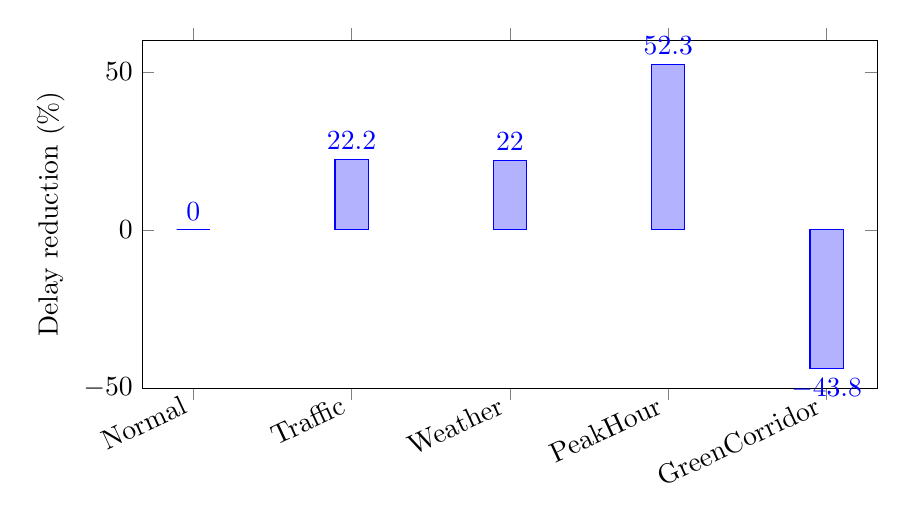
\begin{tikzpicture}
\begin{axis}[
    ybar,
    bar width=12pt,
    width=0.9\linewidth,
    height=6cm,
    ymin=-50, ymax=60,
    ylabel={Delay reduction (\%)},
    symbolic x coords={Normal,Traffic,Weather,PeakHour,GreenCorridor},
    xtick=data,
    nodes near coords,
    nodes near coords align={vertical},
    x tick label style={rotate=25,anchor=east},
    enlarge x limits=0.08
]
\addplot coordinates {
    (Normal,0.0)
    (Traffic,22.2)
    (Weather,22.0)
    (PeakHour,52.3)
    (GreenCorridor,-43.8)
};
\end{axis}
\end{tikzpicture}
\caption{Delay reduction achieved relative to the road baseline across tested scenarios.}
\label{fig:delay-reduction}
\end{figure}

\subsection{Emissions Savings Across Scenarios}
Figure~\ref{fig:emission-savings} shows the corresponding emissions savings percentages.

\begin{figure}[htbp]
\centering
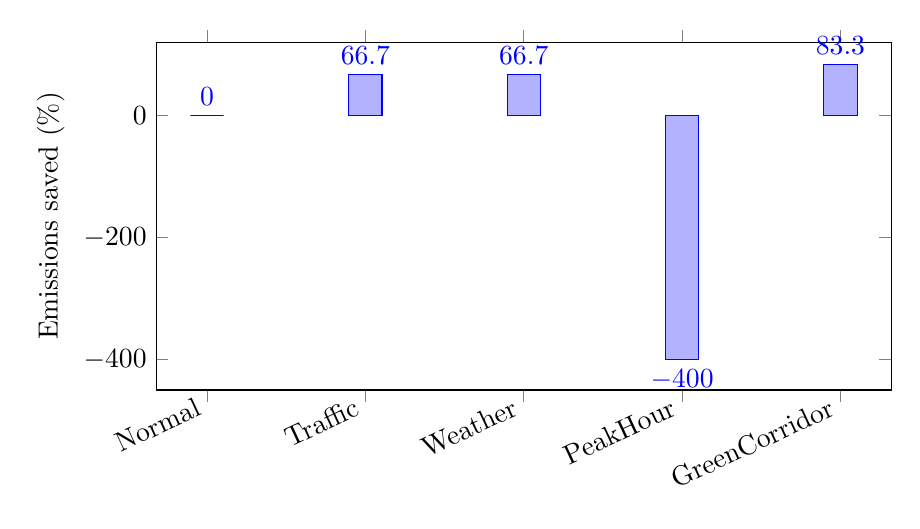
\begin{tikzpicture}
\begin{axis}[
    ybar,
    bar width=12pt,
    width=0.9\linewidth,
    height=6cm,
    ymin=-450, ymax=120,
    ylabel={Emissions saved (\%)},
    symbolic x coords={Normal,Traffic,Weather,PeakHour,GreenCorridor},
    xtick=data,
    nodes near coords,
    nodes near coords align={vertical},
    x tick label style={rotate=25,anchor=east},
    enlarge x limits=0.08
]
\addplot coordinates {
    (Normal,0.0)
    (Traffic,66.7)
    (Weather,66.7)
    (PeakHour,-400.0)
    (GreenCorridor,83.3)
};
\end{axis}
\end{tikzpicture}
\caption{Estimated emissions savings relative to the road baseline. Negative values indicate higher emissions than the baseline.}
\label{fig:emission-savings}
\end{figure}

\subsection{Interpretation for Sustainable Development}
For SDG-oriented transport discussions, the current prototype offers a meaningful but model-based sustainability signal. Emissions are not measured from real vehicle telemetry or carrier fuel data; instead, they are estimated using mode-specific coefficients and edge-level \(\mathrm{CO_2e}\) values embedded in the routing model. Therefore, the reported carbon reductions should be interpreted as \textit{comparative estimated savings under the adopted transport model}. This is still valid for research, especially in early-stage intelligent transport decision-support studies, provided that the assumptions are stated clearly.

\subsection{Practical Meaning of the Results}
From an SDG perspective, the most useful contribution of the current prototype is not that it proves one universal best transport mode. Instead, it demonstrates that route-planning decisions can be made explicitly aware of sustainability metrics. Under conventional planning, route decisions are usually time- and feasibility-driven, while cost and carbon remain afterthoughts. In contrast, the present prototype surfaces the relationship between these variables directly. This is particularly relevant to conference discussions on sustainable infrastructure, responsible consumption, and climate-aware mobility planning.

\subsection{Limitations}
Despite the promising outputs, the current study has several limitations. First, only the road mode uses an external path engine; rail, air, and sea currently depend on a seeded graph network and heuristic service parameters. Second, the emissions values are comparative estimates rather than measured emissions from physical transport assets. Third, the delay dataset is relatively small, containing 200 rows, and therefore the predictive model should be viewed as a prototype-grade estimator rather than a deployment-grade forecasting engine. Fourth, the evaluation scenarios are controlled synthetic scenarios and not a historical archive of real multimodal shipment operations. These limitations should be clearly stated in the paper to preserve the authenticity of the research contribution.

\subsection{Future Work}
Future extensions should proceed in three directions. The first is to integrate timetable-aware or operator-backed rail, sea, and air datasets so that non-road modes become operational routing engines rather than graph abstractions. The second is to improve optimisation logic by incorporating stronger constraint handling for capacities, transfer cutoffs, and shipment scheduling. The third is to improve the emissions model by moving from static coefficients to vehicle-specific or service-specific carbon estimation. Together, these steps would make the system more suitable not only for research demonstration but also for applied pilot deployments.

\section{Conclusion}
This work presented an intelligent routing prototype for multi-modal transport systems that integrates road routing, delay prediction, emissions-aware optimisation, and dashboard-based operational visibility. The implemented system goes beyond single-trip navigation by supporting route comparison under time, delay, cost, and estimated carbon objectives. A FastAPI backend, React frontend, PostgreSQL/PostGIS data layer, OSRM road engine, and Random Forest-based delay service were successfully combined into a coherent research platform.

The current prototype demonstrates that mode selection changes significantly under different operational priorities. Short normal trips remain road-dominant, congestion-heavy and weather-affected scenarios favour rail, highly delay-sensitive scenarios can justify air despite sustainability penalties, and sustainability-weighted long-haul scenarios favour sea transport. These findings indicate that intelligent multimodal selection can provide a useful trade-off analysis framework for sustainable logistics planning.

At the same time, the study has clear limitations. Only road routing is backed by an external routing engine, while rail, sea, and air currently operate through a graph-based research prototype rather than real timetable-aware operator networks. Similarly, carbon savings are estimated through modeled coefficients rather than field-validated fuel or lifecycle measurements. Despite these limitations, the system is sufficiently grounded for research reporting, prototype demonstration, and SDG-oriented discussion on lower-emission freight decision support.

\begin{thebibliography}{99}

\bibitem{matei2021}
O. Matei, R. Erdei, and C.-M. Pintea, ``Selective Survey: Most Efficient Models and Solvers for Integrative Multimodal Transport,'' \textit{Informatica}, 2021, doi: 10.15388/21-INFOR449.

\bibitem{ghaderi2015}
F. Ghaderi and P. Pahlavani, ``A New Multimodal Multi-Criteria Route Planning Model by Integrating a Fuzzy-AHP Weighting Method and a Simulated Annealing Algorithm,'' \textit{The International Archives of the Photogrammetry, Remote Sensing and Spatial Information Sciences}, 2015, doi: 10.5194/isprsarchives-XL-1-W5-203-2015.

\bibitem{shang2021}
X. Shang, K. Yang, B. Jia, Z. Gao, and H. Ji, ``Heuristic Algorithms for the Bi-Objective Hierarchical Multimodal Hub Location Problem in Cargo Delivery Systems,'' \textit{Applied Mathematical Modelling}, 2021, doi: 10.1016/j.apm.2020.09.057.

\bibitem{maneengam2023}
A. Maneengam, ``Multi-Objective Optimization of the Multimodal Routing Problem Using the Adaptive $\varepsilon$-Constraint Method and Modified TOPSIS with the D-CRITIC Method,'' \textit{Sustainability}, 2023, doi: 10.3390/su151512066.

\bibitem{liwang2023}
H. Li and Y. Wang, ``Hierarchical Multimodal Hub Location Problem with Carbon Emissions,'' \textit{Sustainability}, 2023, doi: 10.3390/su15031945.

\bibitem{koohathongsumrit2024}
N. Koohathongsumrit, W. Chankham, and W. Meethom, ``Multimodal Transport Route Selection: An Integrated Fuzzy Hierarchy Risk Assessment and Multiple Criteria Decision-Making Approach,'' \textit{Transportation Research Interdisciplinary Perspectives}, 2024, doi: 10.1016/j.trip.2024.101252.

\bibitem{qiu2021}
B. Qiu and W. Fan, ``Machine Learning Based Short-Term Travel Time Prediction: Numerical Results and Comparative Analyses,'' \textit{Sustainability}, 2021, doi: 10.3390/su13137454.

\bibitem{prakash2024}
S. Prakash, U. Mehta, and B. Sharma, ``Artificial Intelligence-Driven Multimodal Route Planning: Addressing Dynamic Unavailability and Disruptions,'' \textit{IEEE Access}, 2024, doi: 10.1109/ACCESS.2024.3498863.

\bibitem{zhao2024}
S. Zhao and S. Zhao, ``Ship Global Traveling Path Optimization via a Novel Non-Dominated Sorting Genetic Algorithm,'' \textit{Journal of Marine Science and Engineering}, 2024, doi: 10.3390/jmse12030485.

\end{thebibliography}
